%!TEX root = ../dokumentation.tex
\chapter{Basis Konzept}
Die Grundlegende Idee besteht darin die Intelligenz aus dem Roboter herauszunehmen und stattdessen eine intelligente Infrastruktur in eine definierte Umgebung zu integrieren. Dieser Ansatz löst das Platzproblem auf mobilen Plattformen. Auf bzw in Robotern verbaute Rechnersysteme sind primär Platz und Ressourcen-schonend. Die Leistung solcher Geräte ist allerdings sehr beschränkt. Mit dem Auslagern in die Umgebung stehen mehr Platz und somit auch mehr Leistung zur Verfügung. Dies eröffnet zudem andere Lösungsansätze für bekannte Probleme. Gleichzeitig wird die Kommunikation mit der mobilen Plattform deutlich Komplexer, da durch die geschaffene Entfernung Kennwerte wie Latenz enorm an Gewicht zulegen. Aus diesem Grund soll die Basis des Systems auf ROS aufbauen. 
%	\begin{itemize}
%	\item Grundlegende Idee -> Intelligenz aus Roboter herausnehmen in die Umgebung integrieren
%	\item Löst Platzproblem; Auf mobilen Plattformen nur sehr Platz und Energieeffiziente dadurch aber langsame Systeme
%	\item Mehr Platz = Mehr Leistung möglich; ermöglicht andere Lösungsansätze
%	\item Fokus liegt hier nun auf Kommunikation der beteiligten Komponenten
%	\item Grundmechanik auf ROS aufsetzen -> Eventbus -> liefert Basis für Kommunikation und für Eventhandling -> Erweiterungsfreundlich -> sehr gute Doku -> breite Unterstützung
%	\end{itemize}

	\section{Kommunikation}
	Die Kommunikation innerhalb des Systems nutzt die von ROS bereitgestellten Komponenten. Diese nutzen Netzwerktechnologien und bauen auf den Netzwerkstack des Betriebssystems auf. Da bei diesem Projekt die Flexibilität der mobilen Plattform erhalten bleiben soll, wird als Übertragungsmedium \textit{IEEE 802.11} (W-LAN / WIFI) benutzt.
%	\begin{itemize}
%	\item ROS nutzt netzwerktechnologien
%	\item Medium W-LAN -> Flexibel -> Alle Komponenten schon damit ausgestattet
%	\item Kommunikation innerhalb von ROS
%	\item ROS nutzt hierfür Messages in verschiedenen einfach zu definierenden Formaten
%	\end{itemize}

	\section{Eventhandling}
	Das Eventhandling soll über einen zentralen Service innerhalb des ROS-Systems erfolgen. Ereignisse und Nachrichten werden in ROS in so genannten Topics verbreitet. Dieser Dienst soll die relevanten definierten Topics des Systems überwachen und entsprechend darauf reagieren.
%	\begin{itemize}
%	\item Eventhandling über zentralen Service innerhalb des ROS-Systems
%	\item Überwacht fest definierte Topics
%	\item bei Message auf kritischen Topics -> sofortiges Befehl absetzen an mobile Plattform
%	\end{itemize}

	\section{Wahrnehmen der Umgebung}
	Die visuelle Schnittstelle des Systems wird eine Kinect Kamera von Microsoft sein. Diese Entscheidung wurde augrund der sehr guten Dokumentation des Gerätes getroffen. Zusätzlich findet die Kinect eine große Unterstützung in vielen Projekten. Dies geht zweifelsfrei auf die freien Treiber und Bibliotheken zurück. Ein weiterer Grund besteht darin dass nur sehr wenige Geräte sowohl über einen herkömmlichen RGB als auch Tiefensensor verfügen. Zuletzt bietet die Kinect v1 ein sehr gutes Preis/Leistungs - Verhältnis.
%	\begin{itemize}
%	\item Kinect
%	\item gut dokumentiert
%	\item breite Unterstützung durch freie Treiber und Bibliotheken
%	\item RGB und Tiefensensor in einem Gehäuse
%	\item Preis/Leistungs-Verhältnis sehr gut
%	\end{itemize}
	
	\section{Aufbau der Infrastruktur}
	\begin{figure}[H]
	\centering
	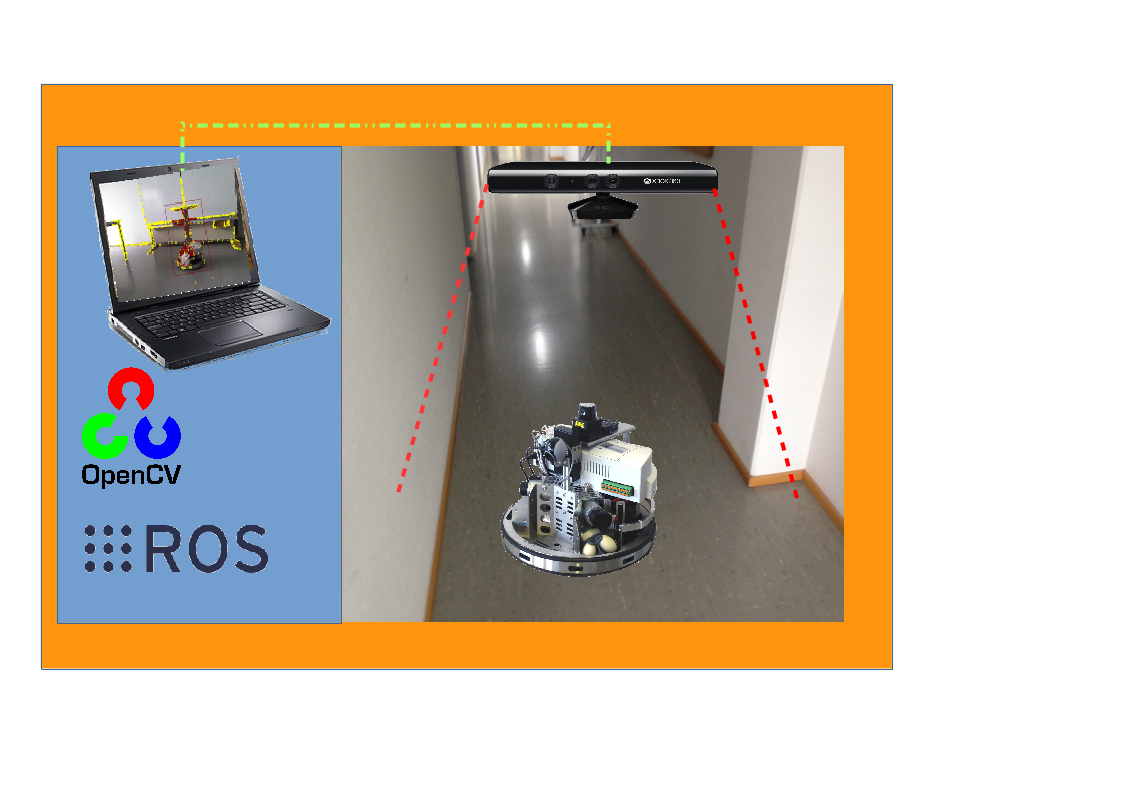
\includegraphics[height=.5\textheight]{../media/infrastruktur}
	\caption{Schematischer Aufbau der geplanten Infrastruktur.}
	\label{fig:infrastruktur}
	\end{figure}
